\newcommand{\note}[1]{\color{red}\textbf{#1}}

\title{P2PSP (Peer-to-Peer Straightforward Protocol)}
\maketitle
\tableofcontents

\begin{abstract}
% Emacs, this is -*-latex-*-

% Abstract

\href{https://p2psp.github.io}{P2PSP (Peer-to-Peer Straighforward
  Protocol)} is an application-layer multicast protocol that provides
real-time broadcasting of media streams in the Internet. The peers
relay the stream split into chunks, using a push communication
model. The data flow is controlled by the source(s) of the stream, and
the peers use a congestion control method based on the relaying of
chunks, only when chunks are received. The topology of the overlay is
dynamic and adapted to the requirements of the physical topology and
startup latency required, which is proportional to the maximum number
of peers in the P2P overlay. In absence of connectivity restrictions
(such as the imposed by NATs) and selfish peers, all peers have a I/O
ratio close to 1, although this ratio can be controlled for each
peer. P2PSP can use unicast and IPM (IP Multicast) communications,
when available.

\end{abstract}

\section{DBS (Data Broadcasting Set)}
\label{sec:DBS}
% Emacs, this is -*-latex-*-

% Data Broadcasting Set of rules (body)

\label{sec:DBS}
% Emacs, this is -*-latex-*-

\label{sec:DBS}

\begin{notex}
  Finished and implemented.
\end{notex}

\acrshort{DBS} is the most basic set of rules. The rest of sets extends or modify
its functionality.

\begin{table}
  \centering
  \begin{tabular}{rl}
    Parameter & Meaning \\
    \hline
    $N^*$  & Maximum number of peers in a team \\
    $C$    & Chunk size \\
    $B$    & Buffer size, in chunks, in the peers \\
    $B'$   & Length of the list of the last $B'$ peers served by the splitter \\ 
    $D$    & Diameter of the flooding tree \\
    $L^*$  & Maximum allowed number of lost chunks \\
    $M$    & Number of monitors \\
    $R$    & Average bit-rate of the media \\
    Variable & \\
    \hline
    $N$    & Number of peers in the team \\
    $t_c$  & Chunk time \\
    $t_r$  & Round time \\
    $t_b$  & Buffering time \\
    $t_p$  & Physical network latency \\
    $t_s$  & Start-up time
  \end{tabular}
  \caption{Nomenclature used in DBS.} %
  \label{tab:DBS_nomenclature}
\end{table}

DBS provides \acrshort{ALM} of a \gls{media} \gls{stream} in an
\gls{unicast} environment. The media is sent by a streaming
\gls{server} (which is an external P2PSP entity), and received by a
\gls{splitter}\note{(see Sec.~\ref{sec:LBS})}~. The splitter divides
the stream into a sequence of \gls{chunk}s of data, and relay them to
a \gls{team} of peers, following a round-robing schema. Each peer of a
team gathers the chunks from the splitter and the rest of peers of the
team, and sends them to at least one \gls{player}\note{Peer should
  run even if no player(s) are connected to it.}~.

\begin{comment}
In single layered streams\footnote{Each layer of a
  scalable stream is received by a different peer attached to the same
  player capable or render scalable media.}, each peer is spawned by a
player (normal users should not run peers directly).
%This system has been described in Fig.~\ref{fig:DBS_system}.
\end{comment}

\begin{comment}
/* quitar: We define the set of teams as
$\{T\}$,
%=\{T^1,\cdots,T^{|T|}\}$,
and enumerate the peers in the team $T$ as $T=\{P_1,\cdots,P_{|T|}\}$. */
\end{comment}


\subsection{Team definition and types of peers}
%%% Local Variables:
%%% mode: latex
%%% TeX-master: "<none>"
%%% End:

\label{sec:team_def}

A team is a set of one or more peers that share the same stream. By
definition, in a team of size one, the only peer is known as a
\emph{monitor} peer. In a team with more than one peer, at least one
of them must be a monitor peer. Monitor peers are instantiated by the
overlay administrator to monitorize different aspects of the
broadcasting, such as, the quality of the rendering of the stream.


\subsection{Feeding the team}
%%% Local Variables:
%%% mode: latex
%%% TeX-master: "<none>"
%%% End:

\label{sec:feeding_the_team}

The splitter divides the stream into chunks of constant length $C$
(see Tab.~\ref{tab:DBS_parameters}), and sends exclusively each
chunk to a different \emph{origin peer}\footnote{In the route that a
  chunk trances inside of the team, the origin peer of a chunk is
  first peer that receives that chunk, i.e. the peer selected by the
  splitter.}, using a round-robin schema. Chunks are enumerated to
distinguish them, and this information is transmitted as a part of a
chunk \emph{header}.

\begin{comment}
More details about the implementation
are available in Fig.~\ref{fig:chunk_generation}.

%$x$, conforming a message
%$c_x=[x,\text{chunk}]$, where
%$x=i \text{mod} \text{Splitter\_DBS.list\_of\_peers}.\text{length}()$.

\begin{figure*}
  %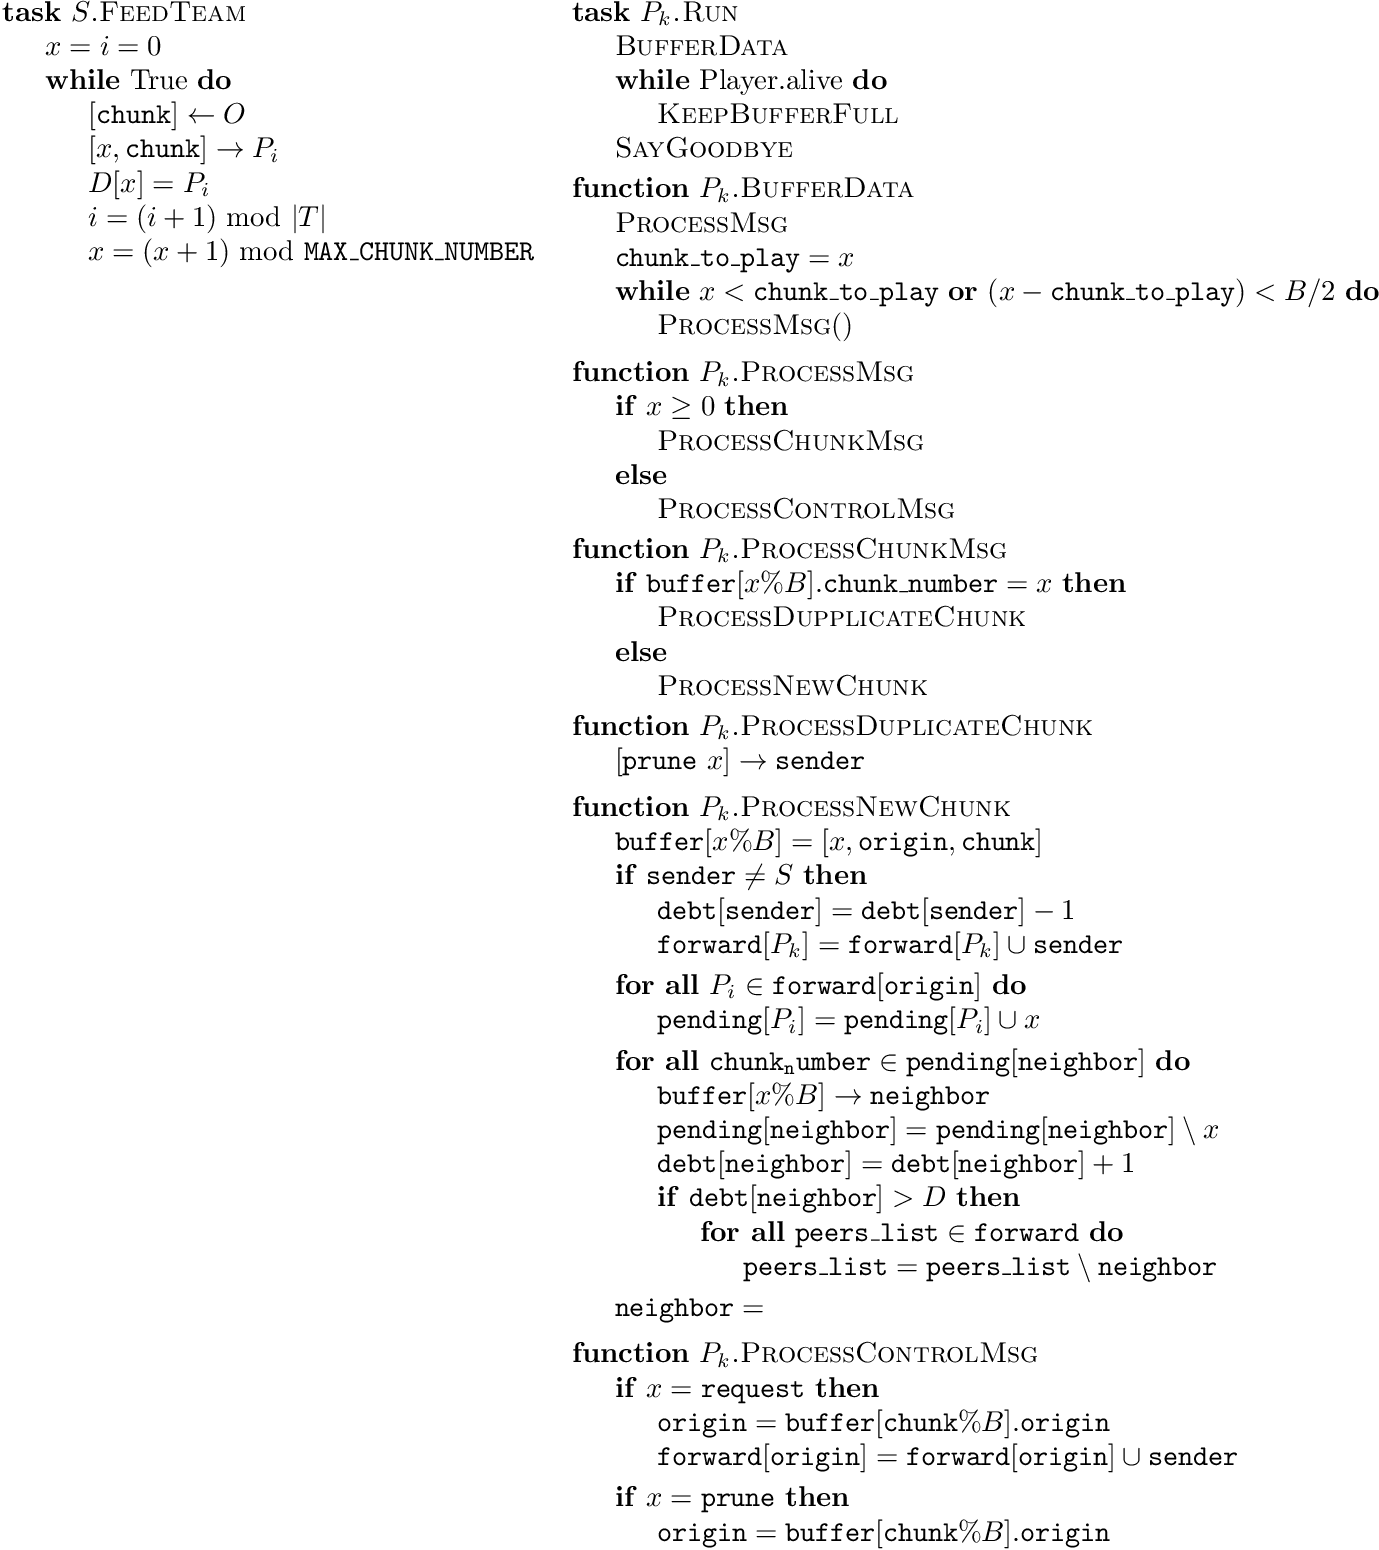
\includegraphics[width=0.75\textwidth]{chunk_generation_and_flooding}
  \fig{500}{5cm}{DBS_splitter_feed} \caption{Chunk
    generation at the splitter and their transmission to the
    team.\label{fig:chunk_generation}}
\end{figure*}
\end{comment}

We define a \emph{round} as the process of transmitting $N\leq N^*$
(see Tab.~\ref{tab:DBS_parameters}) different chunks from the splitter
to a team of $N$ peers. Therefore, for a team of size $N$, the
\emph{round-time} $t_R$ (see Tab.~\ref{tab:DBS_nomenclature}) is $N$
chunk-times. Notice that $t_R$ is generally variable, and depends on
the current number of peers in the team ($N$) and the chunk time
($t_C$) which depends on the chunk size ($C$, see
Tab.~\ref{tab:DBS_parameters}), and the average bit-rate of the media
stream.

The splitter remembers which chunk, of a list of the last $B'$ (see
Tab.~\ref{tab:DBS_parameters}) transmitted chunks, was sent to each
peer of the team. Notice that, in order to remember the chunk that was
sent to each peer in each round, must be hold that $B'\ge N$. \note{See
  \href{https://github.com/P2PSP/simulator/blob/f0c73be1817e7d3b816cc61cd2c8e59b17f9a0e6/src/core/splitter_dbs.py\#L296}{$\text{destination\_of\_chunk}[]$
    in \texttt{splitter\_dbs.py}}.}

\begin{comment}
(in a team) as the time necessary to send two consecutive chunks from
  the splitter (of such team) to the same peer, using the
  round-robing. This time is variable and depends on $|T|$, $C$, and
  the average bit-rate of the media, $A$.
\end{comment}

\begin{comment}
The round-time is defined by:
\begin{equation}
  \cal{r} = \cal{c}N.
  \label{eq:round_time}
\end{equation}
For example, if we use only one team of $N=256$ peers, a chunk size
$C=1024$~bytes, and a video of $1$~Mb/s, the round time is
\begin{displaymath}
  \cal{r} = \frac{1024\frac{\text{bytes}}{\text{chunk}}\times
    8\frac{\text{bits}}{\text{byte}}}{10^6\frac{\text{bits}}{\text{second}}}\times
  256 \approx 2.1~\text{seconds}.
\end{displaymath}
\end{comment}


\subsection{Joining a team}
% Emacs, this is -*-latex-*-

% Joining the Team

\label{sec:joining}

After connecting with a splitter\footnote{A team can be fed by more
  than one splitter in order to introduce redundancy in single-layer
  stream to deal with the loss of chunks, or when using MDC each
  stream description is transmitted by a different splitter.},
incoming peers request (using a reliable communication) to the
splitter the current list of peers in the team $T$. To minimize the
\gls{joining-time}, the peer sends a $[\mathtt{hello}]$ message to
each other peer of the team, in parallel with the reception of the
list. When a peer of the team receives a $[\mathtt{hello}]$, it adds
the sender of the message to the team list\footnote{Peers also updates
  their team list every time a chunk is received from a peer,
  incorporating the sender and the origin of the chunk.} and to a
jagged array of peers called $\mathtt{f}[]$ \note{(see
  \href{https://github.com/P2PSP/simulator/blob/f0c73be1817e7d3b816cc61cd2c8e59b17f9a0e6/src/core/peer_dbs.py\#L491}{$\text{f[]}$
    in \texttt{peer.py}})}. If a peer $P_i$ has an entry
$\mathtt{f}[P_j]=\{P_k\}$, then each chunk received by $P_i$ and
originated at $P_j$ will be forwarded to $P_k$. When an incoming peer
$P_i$ has received the list of peers, its forwarding table has been
initialized to $\mathtt{f}[P_i]=\{T\setminus P_i\}$. Notice that, as
long as the forwarding table contains this information, all the chunks
received from the splitter will be forwarded to the rest of the team,
directly (in one single hop/chunk). So, in absence of communication
constraints, the team will be organized as a full-connected overlay
(see Fig.~\ref{fig:three_topos}-(a)).

\begin{figure}
  \centering
  \myfig{graphics/topologies}{\columnwidth}{800}
  \caption{Different overlay (team) topologies.}
  \label{fig:three_topos}
\end{figure}%
  
%\begin{figure}%
%  \centering
%%  \subfigure[A full-connected overlay.]{%
%%    \label{fig:full}%
%%    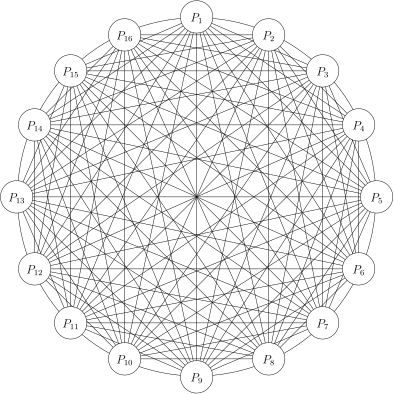
\includegraphics[width=0.45\textwidth]{graphics/full-mesh}}%
%%  \qquad
%%  \subfigure[A star-shaped overlay.]{%
%%    \label{fig:star}%
%%    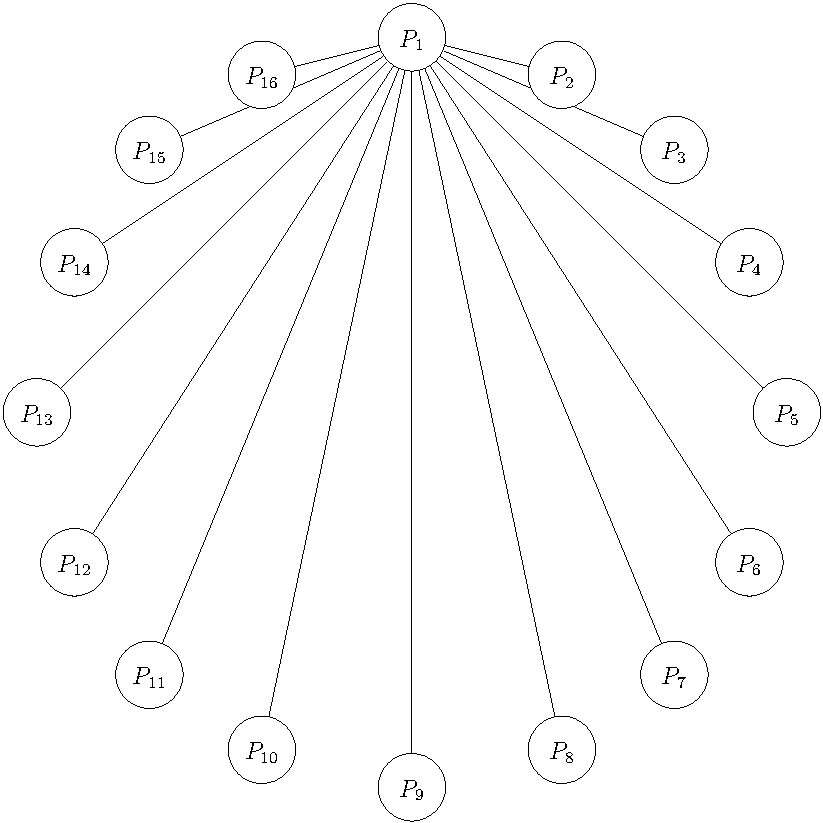
\includegraphics[width=0.45\textwidth]{graphics/star}}%
%\begin{tabular}{ccc}
%  %\subfigure[Full-connected. $\forall P_i\in T, \mathtt{f}[P_i]=T\setminus P_i$]{%
%  %\subfigure{Full-connected. \newline $\forall P_i\in T, \mathtt{f}$[$P_i$]}{%
%  \subfigure{Full-connected}{%
%    \label{fig:full}%
%    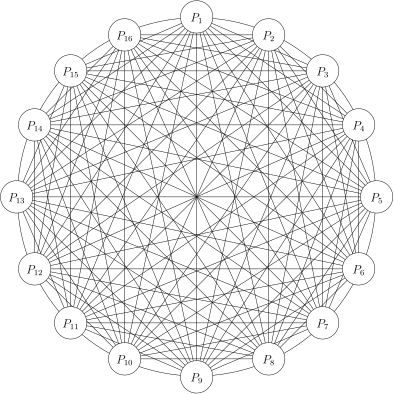
\includegraphics[width=0.3\textwidth]{graphics/full-mesh}}%
%  &
%  \subfigure[Star-shaped.]{%
%    \label{fig:star}%
%    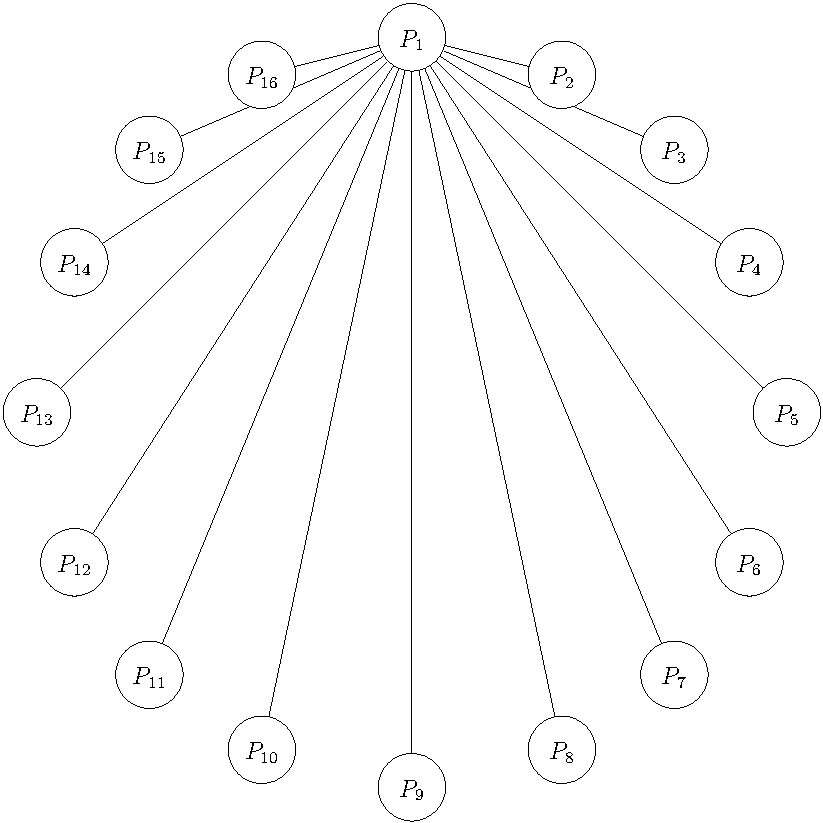
\includegraphics[width=0.3\textwidth]{graphics/star}}%
%  &
%  \subfigure[Ring-shaped.]{%
%    \label{fig:ring}%
%    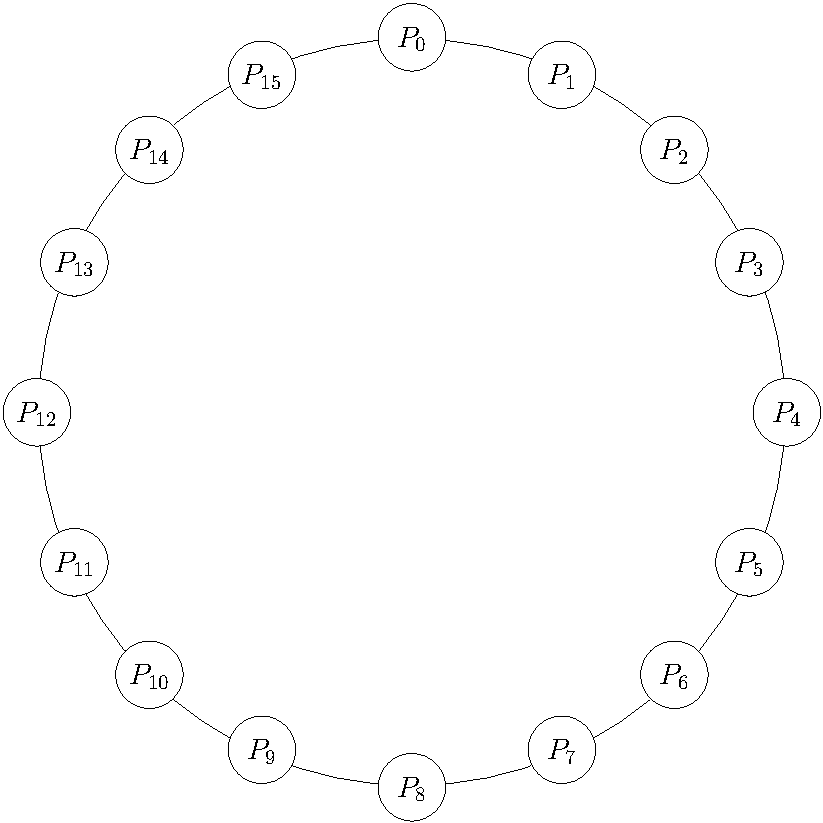
\includegraphics[width=0.3\textwidth]{graphics/ring}}%
%\end{tabular}
%  \caption{Different overlay (team) topologies.}
%  \label{fig:connections}
%\end{figure}

%), initializes
%the table $\mathrm{debt}[]$ (which stores the chunk debts between
%neighbor peers), and (3) sets the variable $\mathrm{neighbor}$ with an
%index to $\mathrm{f}[]$ (see
%Sec.~\ref{sec:chunk_DBS_processing}).

The splitter, in an infinite loop: (1) listens to the incoming peers,
(2) sends to them the list of peers of the team, (3) includes the
incoming peer to the list, and (4) send a copy of the stream to the
team using a round-robing, as a sequence of chunks. Notice that only
those peers that are in the list of peers of the splitter are
considered to be in the team served by such splitter.

\begin{comment}
\begin{figure*}
  %
\includegraphics[width=\textwidth]{joining}
  \fig{1000}{10cm}{joining} \caption{Code related to team
    joining.\label{fig:joining}}
\end{figure*}

The new pseudo-code related to joining a team is describen in the
Fig.~\ref{fig:joining}.
\end{comment}

\begin{notex}
  See \href{https://github.com/P2PSP/simulator/blob/f0c73be1817e7d3b816cc61cd2c8e59b17f9a0e6/src/core/splitter_dbs.py#L296}{$\text{destination\_of\_chunk}[]$ in \texttt{peer\_dbs.py}}.
\end{notex}


\subsection{Buffering chunks}
% Emacs, this is -*-latex-*-

% Buffering chunks

\label{sec:buffering_chunks}

In order to hide the jitter generated by the physical network and the
protocol itself, peers need to store the received chunks in a buffer
during a period of time, before sending them to a player. A chunk with
number $x$ is inserted in the position $(x~\mathit{mod}~2B)$ of the
buffer, where $B$ is the maximum number of chunks that the buffer
stores. In a peer's life, $B$ is a constant specified by the user,
but it is not compulsory that all peers of a team use the same buffer
size.

The buffer is implemented as a circular queue of $2B$ chunks, what is
filled with up to $B$ chunks during the \gls{buffering-time} $t_b$,
which is the main part of the \gls{start-up-time} experienced by
users. Chunks with a higher number (newer chunks) are inserted near of
(depending on the order in which the chunks arrive to the peer) the
head of the buffer. The (received) chunks pointed by the tail of the
buffer $p_p$ (the playing pointer) are sent to the player. This action
is carried out each time a new chunk is received\footnote{DBS does not
  know anything about the content and therefore, about the timing of
  the chunks.}. During the playing process, empty cells in the buffer
(caused by the chunks that have not been received on time) are skipped.

% Hablar de la relación entre B y el tamaño del team. Tal vez, cuando
% se presente la expresión de la latencia en función del grado de
% conectividad. En el caso extremo en que todos los peers se
% conectaran con todos, B >= N^*, el número máximo de peer en el team.


\subsection{Buffering time estimation}
% Emacs, this is -*-latex-*-

% Latency of the streaming system

\label{sec:latency}

%\begin{figure}
%  \centering
%  \vbox{\myfig{graphics/ring}{6cm}{400}}
%  \caption{A ring-shaped overlay.}
%  \label{fig:ring}
%\end{figure}

The start-up time $t_l$ is the latency that the end-user experiments
during the redering of the media. $t_l$, defined as
\begin{equation}
  \label{eq:t_l}
  t_l = t_p + t_b,
\end{equation}
is the sum of the physical
delay $t_p$ and the buffering time $t_b$, where
\begin{equation}
  \label{eq:t_b}
  t_b = Bt_c,
\end{equation}
is the time that has elapsed since the peer receives two chunks
distanced $B$ positions in the buffer, being $B$ the buffer size (in
chunks), and $t_c$ the chunk time (considering $t_c$ a
constant\footnote{If $R$ were time-variying, $t_b$ would be the sum of
  the $t_c$ for each received chunk.}). In other words, the buffering
time is the delay in the rendering of the media required to expect a
seamless playing. Notice that Eq.~\ref{eq:t_b} does not assume that
the chunks fill the buffer in order during the buffering time.

To minimize $t_l$, $t_p$ and $t_b$ should be as small as possible. How
to minimize $t_p$ is out of the scope of this discussion. However, to
minimize $t_b$, we can reduce $t_c$ and/or $B$, but these actions can
carry negative consequences. On the one hand, $t_c$ should be large
enough to reduce the overhead of the headers used by the transport
protocol. On the other hand, if $B$ is too small (for instance $B<N$),
the peer will not have enough space to buffer all the chunks of a
round, causing that incoming chunks to overwrite others before they
can be played due to a low probability of receiving chunks in
order. This problem can also happen even if $N\leq B<2N$, because the
protocol jitter, $\Delta t_b$, that a chunk can experiment is the sum
of the jitter produced by the splitter for this peer, that can as high
as $Nt_c$, and the jitter produced by the flooding of the chunk to the
rest of the team, that also can be has high as $Nt_c$. Notice that
this jitter is the same for two extreme topologies of the overlay: (1)
a full-connected mesh (Fig.~\ref{fig:full}), or (2) a ring
(Fig.~\ref{fig:ring}), when the chunks travel only in one
direction\footnote{Notice that if chunks can travel in both
  directions, we whould have a tree.}. Therefore, in the case of a full-connected mesh, peers have to use a
\begin{equation}
  \label{eq:minimum_B}
  B\ge 2N^*
\end{equation}
in order to avoid the loss of chunks due to high $\Delta t_p$. We will
refeer to $B=2N^*$ as the critical buffer size.

% As a rule of thumb, the larger the buffer size the lower the
% probability of losing chunks, as a consequence of a high $\Delta
% t_p$ (physical jitter).

Lets analyze the buffering time $t_b$ in two interesting cases. Lets
suppose that the number of the first received chunk is $x_1$ and that
the rest of chunks of the buffer of size $B$ are received\footnote{All
  the chunks received with an number smaller than $x_1$ will be
  discarded. Notice also that chunks can arrive in any order.}, being
the chunk $x_{1+B}$ the last one (the best scenario). In this case,
the $t_b$ can still be estimated by Eq.~\ref{eq:t_b}. Lets imagine now
that after receiving $x_1$ the chunk $x_{1+B}$ is received (chunks
$x_2, \cdots x_{1+B-1}$ have been lost or delayed too much), and the
playing starts (probably, with severe artifacts). In this case, $t_b$
also corresponds to Eq.~\ref{eq:t_b}, because the chunk $x_{1+B}$ was
generated $B$ chunk times after $x_1$, and we cannot wait more during
the buffering time if we want to dimension $t_b$. After considering
these two extreme situations, we can deduce that the start-up time
$t_s$ does not depend on the chunk loss ratio during the
buffering-time (for loss ratios smaller than one), but only on $B$,
$t_c$ and $t_p$.

Finally, notice that the time that passes from an incoming peer
request to join a team to a splitter until it accepts the peer, and
the buffering time that the player can require, have not been
considered in this discussion. However, both times should be, in
general, significantly lower than $t_b$, that in the case of P2PSP
corresponds to the $t_s$ that end-users experiment.



\subsection{Chunk flooding}
%%% Local Variables:
%%% mode: latex
%%% TeX-master: "<none>"
%%% End:

\label{sec:chunk_flooding}

\begin{comment}
\begin{figure*}
  %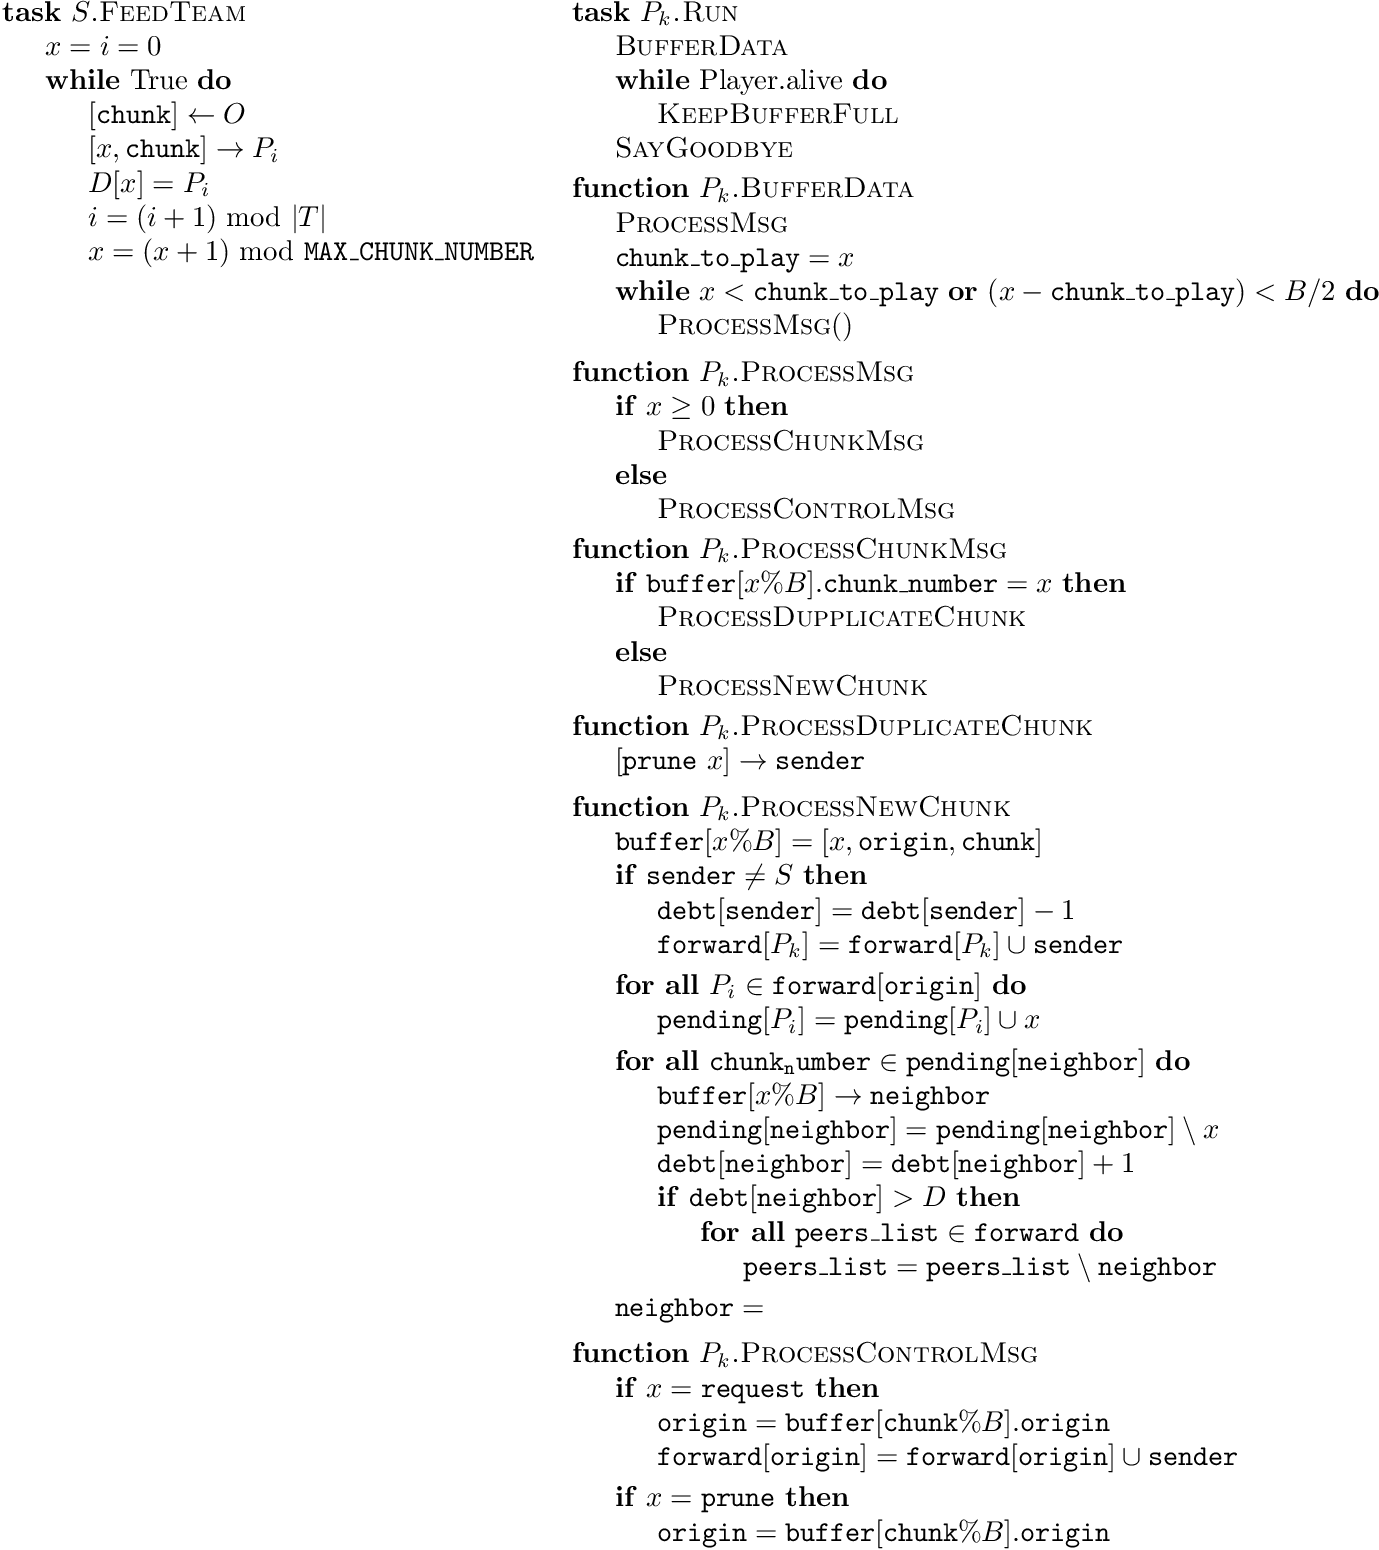
\includegraphics[width=0.75\textwidth]{chunk_generation_and_flooding}
  \imgw{300}{graphics/peer_chunk_flooding.svg}
  \caption{Chunk flooding at peers.\label{fig:peer_chunk_flooding}}
\end{figure*}
\end{comment}

DBS implements a push-based protocol. When a peer receives a chunk, it
can be retransmitted to a large number of neighbors (depending on the
number of different destinations in its forwarding table). Therefore,
even by controlling the chunk rate in the servers\footnote{Using DBS
  the data-flow can not be controlled in the peers or the splitter
  because they don't understand the stream.}, some kind of flow
control must be performed in order to reduce network congestion while
peers perform the flooding.

%Moreover, to achieve an ideal I/O ratio of $1$, peers should send one
%chunk for every received one.

\begin{figure*}
  \centering
  \subfloat[A full-connected overlay.]{\label{fig:full_mesh}
    \vbox{\myfig{graphics/full-mesh}{6cm}{250}}}
  \quad
  \subfloat[A star-shaped overlay.]{\label{fig:star}
    \vbox{\myfig{graphics/star}{6cm}{250}}}
  \caption{In a full-connected DBS team (see Subfig. (a)), all peers
    receive and send the same number of chunks. In a star-shaped DBS
    team such as the shown in the Subfig. (b), $P_1$ should send all
    the chunks of the stream to the rest of the team, except those
    that the splitter has sent directly to the rest of peers.}
\end{figure*}

The congestion (in particular, the one caused by how DBS nodes use the
physical links) may be avoided by means of a basic idea: \textit{if I
have received a chunk, I should send a chunk (not necessary to the
sender)}. It is easy to see that, in a fully connected overlay
(Fig.~\ref{fig:full_mesh}), this allows to control the data
flow. However, in more realistic scenarios (such as those in which
firewalls and symmetric NATS are used), where the physical media
imposes interconnexion constraints, peers can not be ``connected''
with the rest the team, and therefore, if the splitter follows a pure
round-robin strategy, some peers can send more chunks that they
receive (see the Fig.~\ref{fig:star}). In these scenarios, the simple
rule of sending a chunk for each received one does not work.

The previous idea can be adapted to handle a variable connectivity
degree (also called \emph{neighborhood degree}) if each peer uses a
table of lists, $\mathtt{pending}{}$, indexed by the neighbor's
end-points, where each list stores the positions in the buffer of
those chunks that must be transmited to the corresponding neighbor,
the next time such neighbor be selected in the flooding process. Thus,
for example, if $\mathtt{pending}\{P_x\}=\{11,22\}$, chunks found at
positions $11$ and $22$ of the buffer have to be sent to peer $P_x$
(when the pending scheduler used by the peer selects $P_x$).

Notice that using this procedure, more than one chunk can be sent to a
neighbor in a transmission burst, which could congest the switching
devices. However, except in very unbalanced overlays
(Fig.~\ref{fig:star}), the bursts use to be very short (only one chunk
in most of cases). As an advantage, if a burst is produced, all the
chunks of the burst travel between the two same hosts, which usually
increases the performance of the physical routing.

An example of the temporal evolution of a team using this behaviour
has been described in the Figures \ref{fig:team_0}, \ref{fig:team_1}
and \ref{fig:team_2}.

\begin{figure}
  \myfig{graphics/team_0}{4cm}{250} %
  \caption{A team has been created with a single monitor $M_0$
    ($[\mathtt{hello}]$ messages are not shown). Chunks with indexes 0
    and 1 (the time $t$ is measured in chunks-time) have been
    transmitted from the splitter $S$ to $M_0$. $f$ and $p$ represents
    the $\text{forward}[]$ and the $\text{pending}[]$ structures,
    respectively. The chunks stored in the buffer are shown below the
    entity.} %
  \label{fig:team_0}
\end{figure}

\begin{figure}
  \myfig{graphics/team_1}{4cm}{250} %
  \caption{At $t_2$, peer $P_1$ joins the team (the
    $[\mathtt{hello}]$'s are not shown). In $M_0$, $f=\{M_0:[P_1]\}$
    because when $M_0$ receives the $[\mathtt{hello}]$ from $P_1$,
    $M_0$ is the origin peer for all chunks received from $S$ and
    $P_1$ is its neighbor. $P_1$ includes an entry $P_1:[M_0]$ in its
    forwarding table because $M_0$ is in the list of peers received
    from the splitter. After that, when the chunk number 2 arrives to
    $M_0$ from $S$, an entry $P_1:2$ is created in $P\{\}$ for that
    chunk, and this entry is deleted when the chunk 2 is sent to
    $P_1$.} %
  \label{fig:team_1}
\end{figure}

\begin{figure}
  \myfig{graphics/team_2}{4cm}{300} %
  \caption{$P_2$ joins the team. $M_0$ and $P_1$ includes $P_2$ in
    their forwarding tables. The chunk 3 is received by $P_1$ which
    decides to send it to $P_2$. Chunk 3 remains as pending to be sent
    to $M_0$ when the next chunk is received by
    $P_1$.} %
  \label{fig:team_2}
\end{figure}
%  $P_2$ is the origin peer for $M_0$ and $P_1$ because both of them are in the list of peers that $P_2$ receives from $S$.
    
\begin{figure}
  \myfig{graphics/team_3}{4.5cm}{330} %
  \caption{Chunk 4 is received by $P_2$ which relays it to $P_1$, what
    relays chunk 3 to $M_0$.} %
  \label{fig:team_3}
\end{figure}

\begin{figure}
  \myfig{graphics/team_4}{4.5cm}{330} %
  \caption{Chunk 5 is received by $M_0$ which
    relays it to $P_2$.} %
  \label{fig:team_4}
\end{figure}

\begin{notex}
  \begin{figure*}
    \myfig{graphics/team_5}{4cm}{350}
  \end{figure*}
  
  \begin{figure*}
    \myfig{graphics/team_6}{4cm}{380}
  \end{figure*}
  
  \begin{figure*}
    \myfig{graphics/team_7}{4cm}{320}
  \end{figure*}
  
  \begin{figure*}
    \myfig{graphics/team_8}{4cm}{200}
  \end{figure*}
  
  \begin{figure*}
    \myfig{graphics/team_9}{4cm}{280}
  \end{figure*}
  
  \begin{figure*}
    \myfig{graphics/team_10}{4cm}{380}
  \end{figure*}
  
  \begin{figure*}
    \myfig{graphics/team_11}{4cm}{210}
  \end{figure*}
  
  \begin{figure*}
    \myfig{graphics/team_12}{4cm}{210}
  \end{figure*}
  
  \begin{figure*}
    \myfig{graphics/team_13}{4cm}{210}
  \end{figure*}

\end{notex}

%An example of the flooding with congestion control algorithm has been
%show in the Figs.~\ref{fig:team_0}, ...
%Notice that in this example
%all messages are received successfully.
%As can be seen in the example, when a peer $P_k$ receives a chunk,
%$P_k$ floods a number of chunks to one of its its neighbors (obviously,
%except the neighbor sender of the chunk), using round-robin
%schema. The size of this set, what we call $\text{pending}$, depends
%on how many neighbors a peer has.

% Alternative: increment by +1 and decrement by /2

% Alternative: peers keep sorted the neighbors by debt, and the list
% is run from the beginning each time a chunk arrives from the
% splitter.

% Alternative: the debt is only incremented if the relayed chunk has
% been received from the splitter.

% Alternative: if between two consecutive chunks received from the
% splitter (a round), a peer does not receive a chunk from a neighbor
% with origin such neighbor, the peer is removed from the forwaring
% list.

\begin{comment}
In each round, peers check if a chunk have been received from the rest
of peers of the team (${\cal P}_k\in {\cal T}_j)$). If not, peers send
a $[\mathtt{propagate}~{\cal P}_i]$ to one or more (possibly
to the rest of) peers of the team, where ${\cal P}_i$ is the origin peer
of the missing chunk. At this point, the process continues as
described in Section~\ref{dbs:chunk_flooding}.
\end{comment}

\begin{comment}
For each ${\cal P}_k\in N({\cal P}_i)$, ${\cal P}_i$ checks if a chunk
has been received from ${\cal P}_k$. If ${\cal P}_i$ detects that
${\cal P}_k$ has not sent a chunk to it during $L$ consecutive rounds,
performs $N({\cal P}_i) = N({\cal P}_i)\setminus{\cal P}_k$, and stops
sending to ${\cal P}_k$ more chunks.
\end{comment}
\begin{comment}
computes a
``chunk-debt'', denoted by $d({\cal P}_k)$, that is incremented each
time a chunk is received from ${\cal P}_k$ and decremented each time a
chunk is sent to ${\cal P}_k$. If ${\cal P}_i$ verifies that $d({\cal
  P}_k)>D$ (the maximum debt), then ${\cal P}_i$ considers that ${\cal
  P}_k$ is unable to communicate with it, performs $N({\cal P}_i) =
N({\cal P}_i)\setminus{\cal P}_k$, and stops sending to ${\cal P}_k$
more chunks.
\end{comment}

%When peers receive chunks from their splitter, they must flood them to
%their neighbors until the chunks are broadcasted to the whole team
%(Fig.~\ref{fig:chunk_generation_and_flooding}). Lets suppose that
%${\cal P}_k$ receives a chunk. In the case the sender is its splitter,
%${\cal P}_k$ floods the chunk to $N({\cal P}_k)$. However, if the
%sender is a peer ${\cal P}_m\in N({\cal P}_k)$, ${\cal P}_k$ adds
%${\cal P}_m$ to $N({\cal P}_k)$ if ${\cal P}_m$ is a new neighbor, and
%forwards the chunk to the rest of its neighborhood ${\cal P}_n\in
%N({\cal P}_k)\setminus{\cal P}_m$ if ${\cal P}_k$ is in the shortest
%between ${\cal P}_n$ and the origin peer ${\cal P}_i$ of the relayed
%chunk. This will be true if ${\cal P}_k$ is the gateway of ${\cal
%  P}_n$ to go from ${\cal P}_n$ to ${\cal P}_i$. Therefore, a flooding
%with prunning based on shortest path routing is used.

%Peers do not understand the content, but it is
%known that in order to achieve a I/O ratio of 1, peers should send one
%chunk for every received one, on average. To acomplish this, a ${\cal
%  P}_i$ creates a FIFO queue of chunks for each $N({\cal P}_i)$, and,
%for each received chunk, ${\cal P}_i$ forwards a queued chunk from
%each of these queues.

\begin{comment}
A ${\cal P}_i$ forwards one or more chunks if and only if it has
received a chunk. For each received chunk $c_j$, ${\cal P}_i$: 1)
creates a list $l_{c_j}$ with the contents of $N'({\cal P}_i)$, and 2)
sends $c_j$ to $l_{c_j}[0]$ (the first element), and removes
$l_{c_j}[0]$. For each chunk reception, Step 2) is repeated for all
the previously created lists while they are not exhausted.

A solution is a forwarding algorithm based on the following
idea. Peers manage a list of chunks, where every item is a 2-tuple
($c_k$, $P_l$). The field $c_k$ represents the chunk that must be
flooded (if the node that has delivered the chunk is the splitter,
$c_k$ must be relayed towards all the neighbors, otherwise, $c_k$ must
be sent to all the neighbors except the peer that delivered $c_k$),
and the field $P_l$ the last neighbor to which $c_k$ was sent. For
every chunk received, a new tuple is appended to the list of chunks
and the rest of tuples are updated. The field $c_k$ remains constant
but $P_l$ is replaced by the next peer in the list of neighbors for
every received chunk.
\end{comment}


\subsection{Routes discovery and topology optimization}
% Emacs, this is -*-latex-*-

% Routes Discovery and Topology Optimization

\label{sec:routes_discovery}

Chunks can be lost under bandwidth and buffering time constraints (a
chunk is lost when it is time to send it to the player, i.e. when it
is pointed by $p_p$, and the chunk has not been received). Because of
realizing that the chunk pointed by $p_p$ has not been received cannot
recover it on time, peers pre-fetch ``potentially lost chunks'' at the
buffer position $p_p+p_h$, where $p_h\geq 0$ is the pre-feching
horizon. Notice that if $p_h=0$, the pre-fetching is disabled and only
those chunks that really are lost will be requeted. On the contrary,
the higher the $p_h$, the more agressive the pre-fetching.

In this situation, for each (potentially) lost chunk, the peer sends a
$[\mathtt{request}~\text{lost\_chunk\_number}]$ to a random peer of
the team. When a peer $P_i$ receives a
$[\mathtt{request}~\text{lost\_chunk\_number}]$ from $P_j$, $P_i$ adds
$P_j$ to $\mathtt{forward}[P_k]$, where $P_k$ is the origin peer of
the chunk stored in the position
$(\text{lost\_chunk\_number}~\mathit{mod}~2B)$ of its buffer.

Chunks are also requested using a pre-fetching strategy, which has the
objective of reducing the convergence time of the overlay to its
optimal structure (i.e., to reduce as much as possible the loss of
chunks). Peers request those chunks that are in the position $P+O$ of
their buffers, where $O\geq 0$ is an optimization threshold configured
by the user. Notice that if $O=0$, the pre-fetching is disabled. The
higher the $O$, the faster the convergente but also a larger number of
requests messages will be generated, increasing the overhead of the
protocol. Notice also that $O$ can be different between peers and
variable in time.

When request messages are used, redundant routes can be created
between an origin peer and itself, and therefore, some chunks could be
received more than once. Obviously, this is also an overhead that must
be minimized. For this, for each chunk stored in the buffer there is a
set of counters that counts the number of times the chunk has been
received as a duplicate from the corresponding neighbor. When a peer
$P_i$ plays a chunk, $P_i$ send a
$[\mathtt{prune}~\text{duplicate\_chunk\_index}]$ to every neighbor
whose counter is higher than a threshold $D$ (the maximum number of
duplicates per chunk per neighbor, also controlled by the used as a
part of the optimization of the position of its peer in the overlay),
and removes the counter. Neighbors receiving this message from peer
$P_i$ remove the $P_i$ from $\mathtt{forward}[P_k]$, where $P_k$ is
the origin peer of the duplicate chunk.

In Sec.~\ref{sec:chunk_flooding} was introduced the concept of
neighborhood degree. Now, we define this value as the number of
different destination peers for each possible origin that a peer
forwards. For example, if peer $P_i$ forwards chunks from origin $P_i$
to 10 neighbors, the neighborhood degree of $P_i$ for the origin $P_i$
is 10, and if the peer $P_i$ also forwards chunks from origin $P_j$ to 5
neighbors, the neighborhood degree of $P_i$ for the origin $P_j$ is 5.

Considering the rules described before, the neighborhood degrees of
peers can decrease or increase to optimize the topology of the
overlay. An increment in the degree for the origin of a requested
chunk $\text{lost\_chunk\_number}$ in $P_i$ is produced when $P_i$
recives a $[\mathtt{request}~\text{lost\_chunk\_number}]$ from a peer
that is not a neighbor yet. On the contrary, a decrement in the degree
for the origin of a pruned chunk $\text{duplicate\_chunk\_index}$ in
$P_i$ is produced when $P_i$ receives a
$[\mathtt{prune}~\text{duplicate\_chunk\_index}]$ from a neighbor
peer, for that origin.


%\subsection{Overlay topology optimization and the neighborhood degree}
%When a peer $P_i$ is joining the team, it sends a $[\mathtt{hello}]$
to each other peer of the team, which will add $P_i$ to their
$\mathtt{forward}[]$ and $\mathtt{pending}[]$ tables. So, in absence
of communication constraints, the team will be organized as a
full-connected overlay (see Fig.~\ref{fig:full_mesh}).

Peers forward chunks to their neighbors in the order in which the
entries in $\mathtt{pending}[]$ table is accessed, that depends on the
content of the $\mathtt{supportivity}[]$ table. In each round, peers
serve first to the supportive neighbors, fact that will increase their
supportivity in the supportive neighbors, and viceversa. Unsupportive
neighbors are deleted from $\mathtt{forward}[]$ and therefore from
$\mathtt{pending}[]$, decreasing the neighborhood degree.

The neighborhood degree can also grow. Chunks are lost under bandwidth
and buffering time constraints. When a chunk is lost, the peer
requests to receive the rest of chunks from the corresponding origin
peer to a random peer of the known team. If duplicates are generated,
prune messages will remove the slower routes from that origin peer,
generating that the most reliable (and possiblely faster) route to
endure. When this happens, the requesting peer will be added to
$\mathtt{forward}[]$ (and therefore, sooner or later to
$\mathtt{pending}[]$) of the requested peer, increasing its
neighborhood degree.


\subsection{Leaving a team}
\label{sec:leaving}

An outgoing peer must to: (1) say $[\mathtt{goodbye}]$ to the splitter
and the neighbor peers (in this order), (2) relay any pending
(received but yet not sent) chunks, and (3) wait for a
$[\mathtt{goodbye}]$ from the splitter, in this order. In case of
timeout, the leaving procedure is reset.

When a peer of the team receives a $[\mathtt{goodbye}]$, removes the
sender from the $\text{forward}$.

The splitter removes the peer from the list of peers.

\begin{figure*}
  %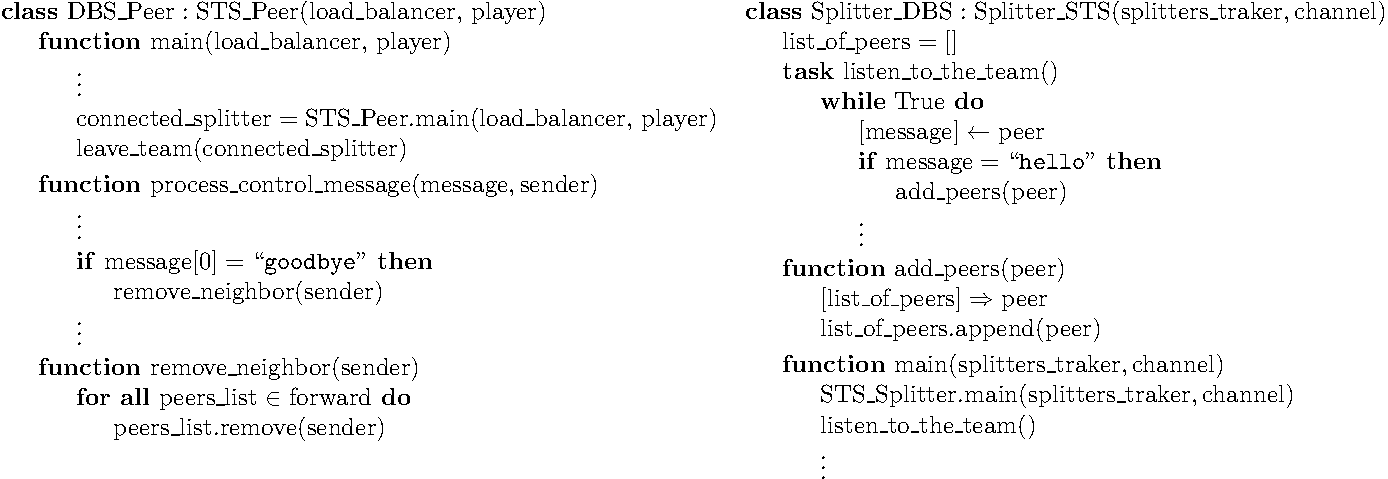
\includegraphics[width=0.55\textwidth]{leaving}
  \fig{400}{4cm}{leaving}
  \caption{Leaving a team.\label{fig:leaving}}
\end{figure*}

All these rules have been describen in Fig.~\ref{fig:leaving}.

\begin{comment}
An outgoing peer $P_o$ (see Fig.~\ref{fig:leaving}) must to: (1) say
$[\mathtt{goodbye}]$ to $S$ and to $T^o$ (in this order), (2)
relay any pending (received but yet not sent) chunks, and (3) wait for
a $[\mathtt{goodbye}]$ from $S$, which performs $T = T \setminus
P_o$. In case of a timeout, $P_o$ resets the leaving procedure,
for a maximum number of times.

When a $P_k$ receives a $[\mathtt{goodbye}]$ from $P_o$, $P_k$
removes $P_o$ from its neighbors set, by running $T^k = T^k
\setminus P_o$.
\end{comment}


\subsection{Free-riding control at the splitter}
% Emacs, this is -*-latex-*-

% Free-riding Control at the Splitter

\label{sec:free_riding_control}

The splitter remembers which chunk, of a list of the last $B'$
transmitted chunks, was sent to each peer of the team. Notice that, in
order to remember the chunk that was sent to each peer in each round,
must be hold that $B'\ge N$. \note{See
  \href{https://github.com/P2PSP/simulator/blob/f0c73be1817e7d3b816cc61cd2c8e59b17f9a0e6/src/core/splitter_dbs.py\#L296}{$\text{destination\_of\_chunk}[]$
    in \texttt{splitter\_dbs.py}}.}

Monitor peers (which are trusted peers) complain to their splitter
with a $[\mathtt{lost}~\text{lost\_chunk\_number}]$ for each lost
chunk. The splitter only considers these type of messages if they come
from a monitor.

%Notice that $L$ will
%tend to be proportional to the number $M$ of monitors, especially if
%those cases where $P_o$ is a gone peer that was unable to transmit the
%$[\mathtt{goodbye}]$ messages.

\begin{notex}
This last functionality has not been implemented, at least, as it has
been explained here. The forget() thread is controlled by a timer, not
by a counter of rounds.
\end{notex}

%Peers also control that at least one chunk is received from a neighbor
%in each round.\footnote{Peers recognize that a new round has started
%  when a new chunk is received from the splitter.} If happens that a
%peer $P_x$ does not receives a chunk from peer $P_y$ between $D^*$
%consecutive rounds, $P_x$ removes $P_y$ of its forwaring table.


\subsection{Free-riding control at peers}
In each round, peers check if a chunk have been received from the rest
of peers of the team (${\cal P}_k\in {\cal T}_j)$). If not, peers send
a $[\mathtt{propagate}~{\cal P}_i]$ to one or more (possibly
to the rest of) peers of the team, where ${\cal P}_i$ is the origin peer
of the missing chunk. At this point, the process continues as
described in Section~\ref{dbs:chunk_flooding}.

\begin{comment}
For each ${\cal P}_k\in N({\cal P}_i)$, ${\cal P}_i$ checks if a chunk
has been received from ${\cal P}_k$. If ${\cal P}_i$ detects that
${\cal P}_k$ has not sent a chunk to it during $L$ consecutive rounds,
performs $N({\cal P}_i) = N({\cal P}_i)\setminus{\cal P}_k$, and stops
sending to ${\cal P}_k$ more chunks.
\end{comment}
\begin{comment}
computes a
``chunk-debt'', denoted by $d({\cal P}_k)$, that is incremented each
time a chunk is received from ${\cal P}_k$ and decremented each time a
chunk is sent to ${\cal P}_k$. If ${\cal P}_i$ verifies that $d({\cal
  P}_k)>D$ (the maximum debt), then ${\cal P}_i$ considers that ${\cal
  P}_k$ is unable to communicate with it, performs $N({\cal P}_i) =
N({\cal P}_i)\setminus{\cal P}_k$, and stops sending to ${\cal P}_k$
more chunks.
\end{comment}


%\subsection{Free-riding control at peers} % Neighborhood dynamics
%\label{dbs:frcp}
%In each round, peers check if a chunk have been received from the rest
of peers of the team (${\cal P}_k\in {\cal T}_j)$). If not, peers send
a $[\mathtt{propagate}~{\cal P}_i]$ to one or more (possibly
to the rest of) peers of the team, where ${\cal P}_i$ is the origin peer
of the missing chunk. At this point, the process continues as
described in Section~\ref{dbs:chunk_flooding}.

\begin{comment}
For each ${\cal P}_k\in N({\cal P}_i)$, ${\cal P}_i$ checks if a chunk
has been received from ${\cal P}_k$. If ${\cal P}_i$ detects that
${\cal P}_k$ has not sent a chunk to it during $L$ consecutive rounds,
performs $N({\cal P}_i) = N({\cal P}_i)\setminus{\cal P}_k$, and stops
sending to ${\cal P}_k$ more chunks.
\end{comment}
\begin{comment}
computes a
``chunk-debt'', denoted by $d({\cal P}_k)$, that is incremented each
time a chunk is received from ${\cal P}_k$ and decremented each time a
chunk is sent to ${\cal P}_k$. If ${\cal P}_i$ verifies that $d({\cal
  P}_k)>D$ (the maximum debt), then ${\cal P}_i$ considers that ${\cal
  P}_k$ is unable to communicate with it, performs $N({\cal P}_i) =
N({\cal P}_i)\setminus{\cal P}_k$, and stops sending to ${\cal P}_k$
more chunks.
\end{comment}


%\subsection{Congestion control}
%\label{dbs:congestion_control}
%%%% Local Variables:
%%% mode: latex
%%% TeX-master: "<none>"
%%% End:

\label{sec:congestion_control}

DBS is a content-unaware push-based protocol, where when a peer
received a chunk, it can be retransmitted to a large number of
neighbors. To avoid network congestion while flooding, sending peers
must perform some kind of data flow-control.

%Moreover, to achieve an ideal I/O ratio of $1$, peers should send one
%chunk for every received one.

Congestion control is performed by means of the basic idea of, {\sl if
  I have received a chunk, I should send a chunk}. It is easy to see
that, in a fully connected overlay, this allows to control the data
flow. However, peers can be ``connected'' with a variable number of
neighbors and therefore, if the splitter follows a pure round-robin
strategy, some peers can send more chunks that they receive.

The previous idea can be improved to handle a variable connectivity
degree. Each peer use an array of FIFO queues, $\text{pending}[]$,
indexed by the neighbor end-points, where each queue stores buffer
positions. Thus, if for example $\text{pending}[P_x]=\{11,22\}$,
chunks found at positions $11$ and $22$ of the buffer have to be sent
to peer $P_x$ when the priority round-robin scheduler used by the peer
select $P_x$ (see Sec.~\ref{sec:chunk_flooding}).


............

in DBS is very simple: if a new chunk is
received, peers forward (using the flooding with prunning algorithm
described in Sec~\ref{dbs:chunk_generation_and_flooding}) each
received chunk to the next peer of their list of peers (following a
round-robin pattern).

%Peers do not understand the content, but it is
%known that in order to achieve a I/O ratio of 1, peers should send one
%chunk for every received one, on average. To acomplish this, a ${\cal
%  P}_i$ creates a FIFO queue of chunks for each $N({\cal P}_i)$, and,
%for each received chunk, ${\cal P}_i$ forwards a queued chunk from
%each of these queues.

\begin{comment}
A ${\cal P}_i$ forwards one or more chunks if and only if it has
received a chunk. For each received chunk $c_j$, ${\cal P}_i$: 1)
creates a list $l_{c_j}$ with the contents of $N'({\cal P}_i)$, and 2)
sends $c_j$ to $l_{c_j}[0]$ (the first element), and removes
$l_{c_j}[0]$. For each chunk reception, Step 2) is repeated for all
the previously created lists while they are not exhausted.

A solution is a forwarding algorithm based on the following
idea. Peers manage a list of chunks, where every item is a 2-tuple
($c_k$, $P_l$). The field $c_k$ represents the chunk that must be
flooded (if the node that has delivered the chunk is the splitter,
$c_k$ must be relayed towards all the neighbors, otherwise, $c_k$ must
be sent to all the neighbors except the peer that delivered $c_k$),
and the field $P_l$ the last neighbor to which $c_k$ was sent. For
every chunk received, a new tuple is appended to the list of chunks
and the rest of tuples are updated. The field $c_k$ remains constant
but $P_l$ is replaced by the next peer in the list of neighbors for
every received chunk.
\end{comment}


\begin{comment}
\subsubsection{Flooding order}
\label{dbs:flooding_order}
As an incentive mechanism~\cite{xu2006analysis}, peers relay received
chunks first to those peers that 
\end{comment}

%neighbors with lower chunk-debts.

\begin{comment}
\subsubsection{Team dynamics}
\label{dbs:team_dynamics}
${\cal P}_i$ adds to $N({\cal P}_i)$ those ${\cal P}_j$ that has sent
to ${\cal P}_i$ a chunk. If $N({\cal P}_i)>K$, periodically, ${\cal
  P}_i$ removes from $N({\cal P}_i)$ the peer with highest chunk-debt
and try to find in ${\cal T}_j\setminus N({\cal P}_i)$ a new peer using
$[\mathtt{hello}]$ messages.
\end{comment}

\begin{comment}
Peers use a buffer $b$ of chunks to hide the jitter generated by the
physical network and the broadcasting protocol. When a peer receives
$C_i$, it performs
\begin{equation}
  b[i~\text{mod}~B] = c_i,
\end{equation}
where ``mod'' represents the modulo operator and $B$ the buffer size
(in chunks). Basically, the buffer represents a sliding window that
moves over the stream synchronizely with the playing because the the
player consumes the chunks at the same chunk-rate the source produces
them.
\end{comment}

%%%%%%%%%%

\begin{comment}

\begin{itemize}

\item In the P2PSP, only monitor peers complains about lost
  chunks. This means that if a chunk that has been retransmitted by a
  peer is lost, it will be only retransmitted to all the peers of the
  team if the destination is a monitor peer and there is a unique
  monitor peer in the team. On the other hand, if the lost chunk was
  traveling from the splitter to a peer, all monitor peers will
  complain and this chunk will be retransmitted to the complete
  team. Therefore, only massively loss chunks will be retransmitted in
  the P2PSP. However, notice that a isolated missing chunk will
  produce negligible artifacts in the playback of one peer. In the
  Chain model, the lost of a chunk is handled between neighbour peers
  which means that all lost blocks should be, a priori, recovered.

\end{itemize}

\end{comment}



\begin{comment}
\subsubsection{Shortest path computation}
\label{dbs:chunk_routing}
\begin{figure}
  %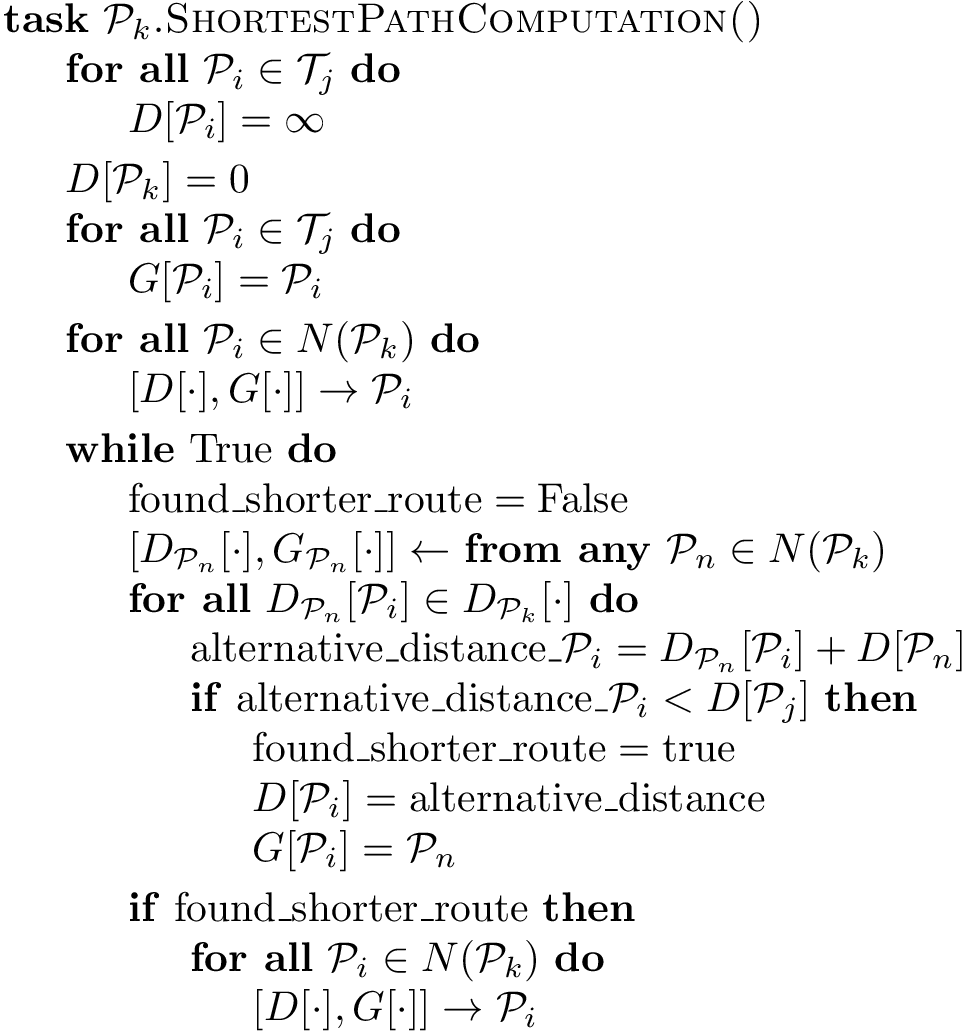
\includegraphics[width=0.35\textwidth]{shortest_path_computation}
  \fig{500}{4cm}{shortest_path_computation}
  \caption{Shortest path computation.\label{fig:shortest_path_computation}}
\end{figure}
The shortest path distances among peers are determined by a variation
of the Bellman-Ford Algorithm~\cite{Bertsekas1987data} (see
Fig.~\ref{fig:shortest_path_computation}), where the cost of the
``links'' between neighbor peers is $1$. Neighbor peers interchange
two vectors $D[\cdot]$ (distance-to-peer) and $G[\cdot]$
(gateway-to-peer) and compute the shortest distances and the (peer)
gateways to (reach) the rest of peers of its team ${\cal T}_j$.

This algorithm is free of routing loops and is not suceptible of the
well known count-to-infinity problem, and therefore always converges
for static teams. These problems do not appear because the routes are 

Each peer ${\cal P}_k$ sends
its vector of distances $D[\forall {\cal P}_i\in T^*({\cal P}_k)]$ and
gateways $G[\forall {\cal P}_i\in T^*({\cal P}_k)]$ to each
neighbor. When this information is received, peers check if shorter
routes can be found to the rest of peers of the reachable team, and if
so, send these vectors again.

The Bellman-Ford algorithm is susceptible of routing loops and the
count-to-infinite problem.


% Hace falta saber desde dónde viene el chunk original (origin peer) y que todos los peers dispongan de los vector-distances de los peers vecinos. Los vector-ditances deben tener tantas entradas como peers existen en el team. Por tanto, cada peer almacena un número de vector-distances igual a su grado de conectividad.


% Supposing that the weight of links between neighbors is 1.
% ¿Cómo sabe un peer que él es el último?
\end{comment}

\begin{comment}
\subsubsection{Generation of the routing tables}
Routing tables has as many entries as peers are in the team. The
routing table of a peer $P_i$ is a dictionary of pairs ($d(P_i, P_j)$,
$P_k$) indexed by the destination peer $P_j$ is a destination peer,
where $d(P_i, P_j)$ is the last measurement of the number of hops (in
peers) between $P_i$ and $P_j$, and $P_k\in N(P_i)$ is the 1-hop peer
that in the shortest-path between $P_i$ and $P_j$. Notice that if
$P_j==P_k$ then $d(P_i, P_j)==1$, which means that $P_i$ and $P_j$ are
directly ``connected''.

When a peer has updated its routing table, it is sent to their
neighbors pyggibacked on a \textsf{chunk} packet. When a peer receives
a routing table, it keeps a copy of it and updates its own routing
table with the new routing information using the Bellman-Ford
Algorithm~\cite{}. The peers have a copy of the routing table of its
neighbors to use it through the chunk routing process (see
Rule~\cite{the_routing_process}.
\end{comment}



\section{FCS (Free-riding Control Set)}
\label{sec:FCS}
%%% Local Variables:
%%% mode: latex
%%% TeX-master: "<none>"
%%% End:

\begin{comment}
Notice that in this example, for the sake of simplicity, a simple
round-robing pending scheduler has been used.  Actually, DBS selects
the $\mathtt{pending}[]$ entries using the supportivity information
gathered from the neighbors. This information is stored in a
$\mathtt{supportivity}[]$ table, which is indexed by the neighbors
end-points. When the list of peers is received from the splitter, all
the peers have the same supportivity. These supportivity values are
incremented each time a chunk is received from the corresponding
neighbor and decremented each time a chunk is received form the
splitter (i.e., in each round). Thus, supportive neighbors will tend
to have a higher supportivity than unsupportive neighbors.
\end{comment}

DBS does not imposes any control over the grade of solidarity of the
peers. This means that selfish peers (or simply peers with reduced
connectivity) can stay in the team thanks to the generosity of the
rest of peers, even if they never achive to deliver a chunk to any
peer of the team. This set or rules preclude this possible behavior,
by impossing a minimum degree of solidarity between neighbor peers.

To know the level of solidarity between neighbor peers, each peer uses
a table of chunk debts, $\mathtt{debt}[]$. Every time a peer $P_i$
sends a chunk to $P_j$, $P_i$ increments $\mathtt{debt}[P_j]$, and on
the contrary, decrements $\mathtt{debt}[P_j]$ when $P_i$ receives a
chunk from $P_j$.

Peers forward chunks to their neighbors in the order in which the
entries of $\mathtt{pending}[]$ are accessed (a round-robing
scheduling in DBS). Considering this, FCS modifies this behavior:
\begin{enumerate}
\item To go through $\mathtt{pending}[]$ in the order provided by
  $\mathtt{debt}[]$, selecting first those entries with a smaller
  debts.
\item To reset the run of $\mathtt{pending}[]$ in each round (when a
  chunk is received from the splitter).
\item If $P_i$ realises that $\mathtt{debt}[P_j]>L^*$, $P_i$ removes
  $P_j$ from $\mathtt{forward}[\forall P_k\in\{\text{team}\cup P_i\}]$
  and $\mathtt{pending}[]$. Notice that this action decreases the
  neighborhood degree of $P_i$ and, soon or later of $P_j$ that will
  consider $P_i$ as unsupportive.
\item In DBS, request messages are sent selecting the destination peer
  at random. In FCS, request messages are sent to those peers with a
  higher debt. Thus, if the insolidarity is produced by a overlay
  topology imbalance (an extreme example is in Fig.~\ref{fig:star}),
  badly connected peers peers could have the chance of mitigating this
  problem by forwarding more chunks to their neighbors.
\end{enumerate}

Using FCS, supportive peers will be served first, incrementing the
QoE of the corresponding peers. On the other hand, those peers with a
higher chunk debt will tend to be unserved if no enough bandwidth is
available. 


\begin{comment}
To achieve this behavior, FCS defines that, if ${\cal P}^j_k$ realises
that $\mathtt{debt}[{\cal P}^j_l]>\mathtt{debt}_{\text{max}}$, then
${\cal P}^j_k$ removes ${\cal P}^j_l$ from ${\cal T}^j_k$. Obviously,
${\cal P}^j_l$ should churn, unless it not interested in playing the
media.

, where those peers with
a low chunk debt are selected first.  Debs are clipped to $\pm
D$. In ideal circunstances, debs should be $0$. Obviously, a high
supportivity means a low debt, and viceversa.

In DBS, the splitter sends to each peer of the team one chunk per
round. On the other hand, the peers can have a variable number of
neighbors. In this context, those peers with a higher degree of
connectivity will forward more chunks than the peers with a lower
degree. So, by definition, peers with a lower connectivity will
forward a lower number of chunks for those peers that it is the origin
peer. In the extreme case, a peer $P_x$ behind a NAT could be
connected only with one external peer $P_y$ which should forward to it
all the chunks except those that receive directly from the
splitter. Obviously, in this case, $\text{debt}[P_x]$ in $P_y$ will
reach $D$ fastly.

Peers will remove as neighbors those peers whose debt reaches $D$
during $D^*$ consecutive rounds.
\end{comment}

\begin{notex}
  The prioritized round-robin neighbor selection has not yet been
  implemented as it has been explained here. The $\text{debt}[]$
  structure exists, but is used for a different purporse.
\end{notex}


\begin{comment}
In each round, peers check if a chunk have been received from the rest
of peers of the team (${\cal P}_k\in {\cal T}_j)$). If not, peers send
a $[\mathtt{propagate}~{\cal P}_i]$ to one or more (possibly
to the rest of) peers of the team, where ${\cal P}_i$ is the origin peer
of the missing chunk. At this point, the process continues as
described in Section~\ref{dbs:chunk_flooding}.
\end{comment}

\begin{comment}
For each ${\cal P}_k\in N({\cal P}_i)$, ${\cal P}_i$ checks if a chunk
has been received from ${\cal P}_k$. If ${\cal P}_i$ detects that
${\cal P}_k$ has not sent a chunk to it during $L$ consecutive rounds,
performs $N({\cal P}_i) = N({\cal P}_i)\setminus{\cal P}_k$, and stops
sending to ${\cal P}_k$ more chunks.
\end{comment}
\begin{comment}
computes a
``chunk-debt'', denoted by $d({\cal P}_k)$, that is incremented each
time a chunk is received from ${\cal P}_k$ and decremented each time a
chunk is sent to ${\cal P}_k$. If ${\cal P}_i$ verifies that $d({\cal
  P}_k)>D$ (the maximum debt), then ${\cal P}_i$ considers that ${\cal
  P}_k$ is unable to communicate with it, performs $N({\cal P}_i) =
N({\cal P}_i)\setminus{\cal P}_k$, and stops sending to ${\cal P}_k$
more chunks.
\end{comment}



\section{IMS (Ip Multicast Set)}
\label{sec:IMS}
% Emacs, this is -*-latex-*-

\label{sec:IMS}

\begin{notex}
  Finished and implemented. IMS modifies the functionality of DBS.
\end{notex}

IMS is available by default in LANs (Local Are Networks) and VLANs
(Virtual LANs)~\cite{shabtay2011ip}, but not in the global
Internet~\cite{Comer1}. IMS runs on the top of DBS and provides
efficient native IPM, where available.

All peers in the same LAN or VLAN have the same network address. When
a joining peer $P_i$ receives the list of peers from its splitter,
first checks if there are neighbors in the same subnet. For all those
peers, $P_i$ uses the IP address $\mathtt{224.0.0.1}$ (all systems on
this subnet), (default) port $\mathtt{1234}$, to multicast (only) the
chunks received from the splitter. Therefore, all peers in the same
local network communicate using this multicast group address and
port. The rest of external peers will be referenced using their public
end-points.

\begin{comment}
\subsubsection{Listening IMS}
\label{imp:listening}
By default, all peers listen to $\mathtt{224.0.0.1}$ (All Systems on
this Subnet), port $\mathtt{1234}.

\subsubsection{Joining the team}
\label{ims:joining}
Two peers in the same LAN share the network address. When an incomming
peer ${\cal P}_i$ receives the list of peers, checks if there are
peers in the same LAN. For those peers, ${\cal P}_i$ use the end-point
$\mathtt{224.0.0.1:1234}$.

In IMS, peers
star joining the team as in DBS. However, when a ${\cal P}_i$ receives
a $[\mathtt{hello}~{\cal P}_i]$ from an incomming ${\cal P}_N$, ${\cal
  P}_i$ checks if the source IP address corresponds to the same
LAN. If this is true, ${\cal P}_i$ replies with a
$[\mathtt{hello}~{\cal P}_x]$, where ${\cal P}_x$ is the end-point of
a multicast group selected by ${\cal P}_i$ (if this is not the first
time ${\cal P}_i$ receives a hello from the same LAN, the previous
${\cal P}_x$ is selected). Then ${\cal P}_N$ sends a
$[\mathtt{neighborhood\_request}~{\cal P}_x]$ to ${\cal P}_x$ that, if
received by ${\cal P}_i$, replies with a
$[\mathtt{neighborhood\_accept}~{\cal P}_x]$ to ${\cal P}_x$. Notice
that ${\cal N}({\cal P}_i)$ remain constant (except in the first IMS
iteration where ${\cal P}_x$ is added) and that ${\cal N}({\cal
  P}_N)\cup={\cal P}_x$. None message is sent from 

\subsubsection{Leaving the team}
\label{ims:leaving}

A incomming peer ${\cal P}_N$ 

% What is P2PSP and what makes it special
In this context, we propose P2PSP (Peer-to-Peer Straightfoward
Protocol), an application-layer multicast solution based on the P2P
communication paradigm. Like IP multicasting, in P2PSP it holds that:
(1) there is only a source of data (the so called \emph{splitter}) and
a dynamic group of destinations (the \emph{peers}), (2) only one copy
of the data is sent by the splitter, (3) a ``best-effort''
transmission service is provided, and (4) the nodes (splitter and
peers) do not have knowledge about the transmitted content. Unlike IP
multicasting, in P2PSP: (1) the splitter is the only source, (2) the
nodes know each other, and (3) the network infrastructure only needs
to provide a unicast transmission service (multicasting is achieved by
the nodes at the application-layer level building a overlay
network). However, notice that as a consecuence of that the
communication model used in both systems is virtually the same, P2PSP
can use IP multicasting when this facility is available. As it will
be shown in the evaluation of P2PSP, both protocols (P2PSP and IP
multicast) have a similar performance in terms of bandwidth and
latency.

IMS defines the behaviour of those nodes that can communicate between
them using IP multicast.

\subsubsection{Using IP multicast}
By definition, peers that share the same network address (for example,
peer that are behind the same NAT device) can use IP multicast to
communicate. One of the peers of the multicast group (the oldest one)
works as a bridge between the ``unicast'' and the ``multicast''
subteams. When this peer receives a [\textsf{hello}] from a new peer
that is in the same subnetwork, it selects a multicast channel (IP
address and port) and sends this information to the incomming
peer. Only the bridge peer (the first peer of the ``multicast
subteam'' in joining) is taken into account for the rest of the team
and the splitter. Only the bridge receives chunks from the splitter
and its ``unicast'' neighbors, and this peer is in charge of
retransmitting them to the multicast group.

When leaving, ``multicast'' peers only need to send a
[\textsf{goodbye}] to the splitter and the bridge, which is the only
peer in their lists. The bridge store in its list of peers the
multicast channel, but the \textsf{chunk\_debt} counter is never
incremented.

\subsubsection{Chunk buffering}
Each peer stores the received chunks in a buffer before play them.
The buffer size $B$ in chunks is equal to the expectable (physical)
network's jitter. If $V$ is the average bit-rate of the media
(measured in bits/second), the buffering time is
\begin{equation}
  T = C/V*B.
  \label{eq:buffering_time}
\end{equation}

\end{comment}



\section{LRS (Lost-chunk Recovery Set)}
\label{sec:LRS}
LRS extends DBS (or an extension of it) to retransmit massively-lost
chunks. LRS should be implemented if error-prone communications are
expected, specially if these channels are used by the splitter. LRS is
based on the use of monitors (see Procedure~\ref{dbs:frcS}). The idea
is: ${\cal S}^j$ will resend lost chunks to one or more the monitors
when all monitors in ${\cal T}^j$ report their loss. To increase the
probability of receiving on time the resent chunk (by normal peers),
monitors halves the number of chunks in their buffers in relation to
common peers. LRS only modifies the behavior of ${\cal S}^j$ and the
monitors. Normal peers implement DBS (or its extension).

\begin{comment}
LRS should be used when it is expected to have loss-prone
communication links or when the bit-rate of the stream exceeds the
uploading capacity of the nodes. Notice that the impact of using LSR
for normal peers is null.

P2PSP relies in UDP to transmit the chunks, and obviously, packet
losses can happen. The impact of a packet loss in the QoS provided
depends on where the packets are lost and who lost it. If a packet is
lost in its trip between the splitter and a peer, this packet will be
missed by all the team.

\subsubsection{Monitor peers}
The overlay administrator can create some special peers called, in
short,\emph{monitors}. These peers are introduced to the rest of peers
of the team as normal peers and behave like the rest of well-intended
peers, churn included. Monitor peers can be asked by the splitter to
check whether the operation of the team has and is been correct.

\subsubsection{Selfish peers rejection}
Another functionality of monitors is to tell the splitter which chunks
have not been received on time (the consequence of receiving a lost
too late is the same than not receiving it never). The splitter
memorizes which chunk has been sent to each peer in the current
round. If all monitors reports that a chunk has been lost, the
splitter can determine which peer has been in charge of broadcasting
that chunk and take note of this. If this problem happens a given
number of times, the splitter can expell the unreliable peer from the
team by stop sending to it futher chunks.

\subsubsection{Lost chunk complains} A chunk is considered as lost when
it must be played and the corresponding cell in the buffer is empty
(there is no chunk inside). More specifically, monitors send to the
splitter a [\textsf{lost chunk index} $x$] loss-report message when a
chunk with index $x==\mathsf{chunk}.\mathrm{chunk\_index}$ is lost.

\subsubsection{Retransmission of lost chunks}
Using these complaining messages, the splitter considers that the
chunk stored in the cell $x \% M$ has been lost if the number of
complains is equal to the current number of monitors in the team. In
this case, the splitter resends the lost chunk to a peer selected
randomly.

\subsubsection{Early complaining}
In order to LRS works properly, monitors must identify the lost chunks
before than the rest of peers (otherwise, the resent chunks could
arrive late to the normal peers). A simple way to achieve this is by
halving the buffer (size, measured in chunks) of the monitors. Thus,
when a monitor is reporting a lost chunk, the rest of normal peers
should be expecting to receive this chunk approximately in the middle
of their buffers, and the resent chunk should be received just on
time.
\end{comment}

\begin{comment}

  The P2PSP relies on the UDP as the transport protocol and, obviously,
packet losses can happen. The impact of a packet loss in the QoS
offered by the team depends on where the packet is lost. If the packet
is lost in the trip between the Splitter and a peer, this packet will
be missed by all the peers of the team, included the monitor
peers. However, if the packet is loss in the trip between two peers,
only the destination peer will loss the chunk. Obviously, this last
situation is less harmfull than the firt one.

Only monitor peers tell the Splitter which chunks have not been
received on time. More specifically, a monitor peer $P$ sends to the
Splitter a \texttt{[lost chunk index $x$]} loss report message when a
chunk with chunk-number $x$ has been lost. Using this information, the
Splitter can enumerate the number of times that a chunk has been
lost. In this framework, the LRS module defines that the Splitter
resend a lost chunk stored in the location $x~\text{mod}~M$ of its
buffer of chunks if the number of losses is equal to the number of
monitor peers. The selected peer to resend this block will one of the
monitor peers.

Notice also that, in this case, monitor peers should become aware of a
chunk loss some time before of that the rest of peers of the team send
it to their players, in order to have enough time to resend the lost
chunk from the monitor peer to the rest of peers of the team. A simple
technique is send \texttt{[lost chunk index $x$]} lost report messages
from the monitor peers to the Splitter when the $x$ chunk is missing
at the half of the buffer. Thus, when a monitor peer realizes that a
chunk could have been lost, the rest of peers are receiving those
chunks that are approximately in the middle of their buffers. Now, if
the buffer if large enought, the resent chunks should be received on
time. This implies also that, if the LRS module is implemented, the
buffer size should be doubled and therefore, it holds that
\begin{equation}
  B \leq 2|T|.
\end{equation}

\end{comment}



\section{ACS (Adaptive Chunk-rate Set)}
\label{sec:ACS}
% Emacs, this is -*-latex-*-

\label{sec:ACS}

\begin{notex}
  Unfinished. This set is incompatible with FCS (see
  Sec.~\ref{sec:FCS}).
\end{notex}

ACS modifies the functionality of DBS.

Basically, ACS relaxes the peer's uploading requirements imposed by
DBS. ACS is based on the idea of using the information that the
splitter knows about the number of chunks that each peer has lost (see
Sec.~\ref{sec:free_riding_control}), in order to send to the more reliable peers
a higher number of chunks. In other words, ACS adapts the round-time
of each peer to its capacity, in such a way that the higher the
capacity, the lower the \gls{round-time}. \leorem{Si tiene qie mandar más, ¿cómo va a tener menor round time?}

ACS should be used if we want some peers to \leochange{put}{contribute with} the uploading
capacity than others cannot provide. A possible situation could be
when we want to mix the CS and P2P models, sending more chunks from
the contents provider's hosts to the users's peers, with the
objective, for example, of incrementing the QoS. Because monitors
should lost a minimum number of chunks (supposedly the hosts of the
contents provider should have enough capacity), the ratio of chunks
emitted by the contents provider's hosts can be controlled if a high
enough number of monitor peers (the more monitors, the higher the
ratio). \leo{\hl{leo:} me lo explique mejor.}

Notice that ACS only affects the behavior of the splitter.

\begin{comment}
In most overlay configurations (which should exhibit a full-(or
nearly-full) connected topology), all nodes should transmit exactly
the same number of chunks. This that can be considered a disadvantage
in some situations such as for example, in a ``pay-per-view''
streaming service where the QoS must be guaranteed to all users, even
if they can not send as fast as they receive.

\subsubsection{Uploading capacity estimation}
In full-connected teams, the number of chunks that a peer must
retransmit depends on the number of chunks that the peer receives from
the splitter. Moreover, the splitter can estimate the effective
uploading capacity of the peers by checking the number of times that a
peer has lost a chunk. This estimation can be used to maximizing the
QoS by assigning a different chunk-rate to each peer, depending on its
estimated capacity. In other words, if a peer does not loss chunks,
then its chunk-rate will be increased and viceversa.

\subsubsection{Adaptive chunk-rate (round-robin) scheduling}
By default, the round cycle (the frequency that the splitter sends a
chunk to a peer) of all peers is the same. ACS alters this by using,
for a peer $P_i$, a team cycle proportional to the packet-loss-ratio
of $P_i$. While $P_i$ is lossing chunks, the splitter will send to it
less chunks and will send more chunks to the rest of the team. If the
rest of the team can assume the extra transmission capacity that $P_i$
can not afford, the overlay will be stable.
\end{comment}

\begin{comment}
  All nodes of a team (peers and Splitter) that implements only the DBS
transmitt exactly the same amount of media, which basically imply that
if a peer can not fulfill this requirement it will be thrown off the
team. This could be considered too demanding in some specific
configurations, such as a team of colleagues that want to share a
content regardless of who spends more transmission bandwidth or in PPV
(Pay-Per-View) systems where the stream must be guaranteed to those
users that have paid for receiving the stream.

The number of chunks that ultimately a peer must retransmit depends
exclusively on the number of chunks that the peer receives from the
Splitter. Besides, the Splitter knows the performance of the peers of
the team for the task of retransmitting the chunks by checking the
number of times that the peers has lost a chunk. This knowledgment
could be exploited by the Splitter to maximize the profiting of the
team capacity by assigning a different chunk-rate to the peers
depending on their reliability. In other words, if a peer does not
loss chunks then a higher number of chunks is sent to it than to the
rest of them.

By default, as a consequence of the use of the Round-Robin scheduler
(see Rule~\ref{rul:round-robin}) and supposing a constant bit-rate
encoded media, the Splitter sends a chunk to each peer almost
periodically. Moreover, peers use the reception of a chunk from the
Splitter as a timing event to decide when to switch from the
congestion avoidance control mode (see
Rule~\ref{rul:congestion_avoidance_mode}) to the burst mode (see
Rule~\ref{rul:burst_mode}). Taking into account all this information,
the ACS proposes an adaptive Round-Robing scheduler in which the
sending period of a chunk from the Splitter to a peer $P$ is
proportional to the packet loss ratio of $P$. For example, lets
suppose that peers $P_1$, $P_2$ and $P_3$ belongs to the same team and
that in the last period of time $P_1$ has not lost chunks, $P_2$ has
lost 2 chunks and $P_3$ has lost one chunk. In this situation, the
next 7 chunks will be transmitted following the progression: $P_1,
P_1, P_3, P_1, P_1, P_2, P_3$, if we also suppose that the peers are
stores in the list of peers of the Splitter in order.

\end{comment}



\section{MCS (Multi-Channel Set)}
\label{sec:MCS}
% Emacs, this is -*-latex-*-

\label{sec:MCS}

\begin{notex}
  Unfinished.
\end{notex}

When using MDC~\cite{baccichet2007content}, SVC~\cite{chu2009auction},
or for emulating the CS model, it can be interesting for peers to
belong to more than one team. To implement MCS, peers must replicate
the P2PSP modules (DBS at least) for each team (channel), except the
buffer.

The use of MDC is trivial: the higher the number received descriptions
(channels), even partially, the higher the quality of the
playback. However, when transmitting SVC media, peers should
prioritize the reception of the most important layers.

When a peer belongs to more than one team, and the teams broadcast exactly
the same stream (the same chunks and headers), it could move between
teams seamless (without losts of signal).

A pure CS service could be provided if the corresponding splitter
announces one empty team and sends each chunk so many times as teams
(with one peer/team) there are.



\bibliography{networking,P2P,streaming,misc,simulcasting,SVC,MDC}
